\section{System/Subsystem Design Description}
Aan de camera zit een aantal eisen. Het meest voor de hand liggende eis is dat de resolutie hoog genoeg moet zijn
om bepaalde objecten te kunnen herkennen. Dit is niet de enige eis, zo moet de camera ook kleur kunnen herkennen 
en modulair zijn. Deze camera zal aangesloten moeten worden aan een microcontroller 
zodat de fotos die de camera maakt bewerkt kan worden. Dit betekent dat de microcontroller krachtig genoeg moet zijn 
om fotos op te vragen, verwerken en berekeningen erop uitvoeren. Ook moet hij vervolgens de verwerkte data doorsturen 
naar een centrale server. Dit betekent dat er een manier moet zijn op de microcontroller om deze data te verzenden.
Dit zijn de hardware eisen aan de camera kant, als dit allemaal voldaan wordt is het mogelijk om de camera te 
gebruiken voor de simulatie van bijen.


Uit onderzoek is gebleken dat de Picam V2 voldoet aan de eisen die is gesteld bij de SSS. 
Om deze reden hebben wij voor deze camera gekozen. Elke moderne webcam zou werken maar communicatie met een 
microcontroller wordt onnodig ingewikkeld. Ook zijn deze webcams van een hogere prijsklasse.
Als er gekozen wordt voor een Picam voor de camera, is het uiteraard gebruikelijk om dan een raspberry pi 
te gebruiken als microcontroller. Dit is de enige microcontroller die plug and play werkt met een Picam. 
Vervolgens wordt er gekeken naar de eisen van de Pi, en er is gebleken dat deze eraan voldoet. 
De Pi 4 is krachtig genoeg om afbeeldingen te verwerken en heeft een ingebouwde bluetooth module 
om deze data weer op te sturen naar de server. Dit is dus waarom er gekozen is voor een Raspberry Pi 4.

\subsection{System wide design decisions}
In dit hoofdstuk worden, zoals de tital al verraad, de design decisions behandeld. Hieronder vallen bijvoorbeeld 
input/outputs van het systeem, gedrag keuzes en andere onderdelen die voor het gehele systeem gelden


\subsubsection*{Camera}

\subsubsection*{Server}
asd
\newline

\subsubsection*{Simulatie}
    \begin{center}
    \hspace*{-3.5cm}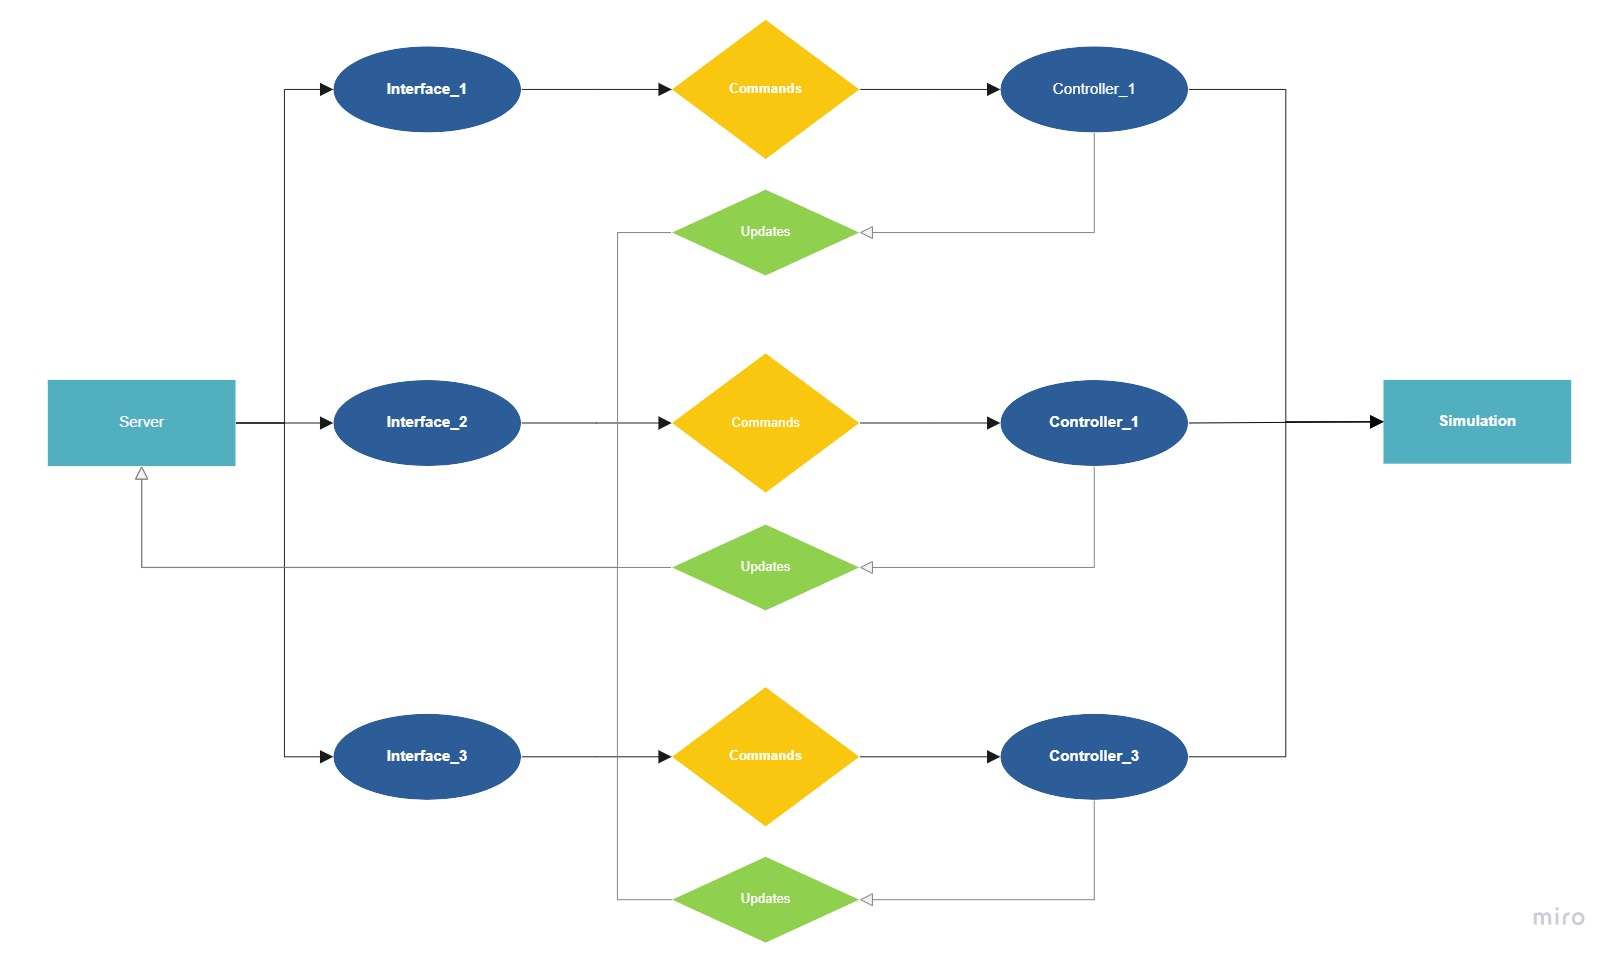
\includegraphics[width=1.6\textwidth]{../IMAGES/Simulation Interaction.jpg}
    \end{center}
    Het diagram hierboven weergeeft de communicatie tussen de simulatie en de server. In de simulatie
    wordt het gedrag van bijen met behulp van 3 ontworpen drones gesimuleerd. Om dat mogelijk te maken
    zijn voor de input en de output de volgende ontwerp keuzes gemaakt: \\
    
    \begin{description}\setlength{\itemindent}{0.1cm}
        \item[INPUT:] \hfill
        \begin{enumerate}
            \item De input voor de simulatie is altijd een opdracht naar een controller. Deze opdracht is een
            actie die een drone moet uitvoeren waarbij een positie meegegeven wordt  naarr de volgende verplaatsingsstap.
            Dit wordt mogelijk gemaakt door te communiceren tegen een opgebouwde interface. Deze 
            interface communiceerd dan vervolgens tegen een controller die een gesimuleerde drone bestuurd.
        \end{enumerate}
        \newpage
        \item[OUTPUT:] \hfill
        \begin{enumerate}
            \item De output bij deze simulatie is verplaatsing van de gesimuleerde drone naar een geplannde positie.
            \item Daarnaast is er ook een andere continue output van de simulatie. Dat is een bericht die afkomstig 
            is van een controller. Een controller stuurt om de bepaalde tijd een bericht naar de server met 
            de informatie over de positie van de bestuurde drone.
        \end{enumerate} 
        
        
    \end{description}

    \newpage
\subsection{System architectural design}


\subsubsection*{System components}
Diagram met hardware en software componenten van het gehelen systeem en de relatie tussen deze onderdelen